\chapter{Transformación de \emph{Legendre}}

	
\begin{tikzpicture}
	\fill [left color=red!50, right color=teal!50] (0,0) rectangle (6.5,.1);
	\fill [left color=teal!50, right color=blue!50] (6.5,0) rectangle (11.5,.1);
	\end{tikzpicture}
	
\vspace{10mm}
\begin{adjustwidth}{50pt}{50pt}
\begin{ejemplo}
La transformada de Legendre es una pieza clave para estudiar el \emph{formalismo hamiltoniano}. Es un mecanismo matemático que se usa, además de en mecánica teórica, en termodinámica.
\end{ejemplo}
\end{adjustwidth}
\vspace{5mm}

\section{La tranformada de \emph{Legendre}}

Una función $f(x)$ almacena información. \emph{Legendre} se preguntó si podía inventarse algún procedimiento que pase a una nueva función $g$, con una nueva variable $p$, tal que la información que estaba en la función original $f$ también esté en la nueva función $g$ y, aún más, si volvemos a efectuar el procedimiento recuperemos la función $f$ original.

Esquemáticamente, llamando $\ \boldsymbol {\hat{A}} $ a la operación a efectuar (procedimiento o transformada de Legendre), 

$$\subrayado{ \boxed{ \ \boldsymbol{ f(x) \qquad \underrightarrow{\quad \hat{A} \quad} \qquad g(p) \qquad  
\underrightarrow{\quad \hat{A} \quad} \qquad f(x) } \ }}$$

Dada $\ f(x)\ \, , \ $ construimos $\quad \hat A \ f(x) \ = \ f'(x)\cdot x \ - \ f(x) \ = \ \left[ x\ \displaystyle \dv{x} -1 \right] \ f(x)$

En general, la variable no tiene por que se $x$, llamémosla $\ \ \textcolor{red}{var.\ origen} \, , \ $ así,

\begin{equation}
 \ \boldsymbol{
\hat A \ = \ \displaystyle \left[ \textcolor{red}{var.\ origen}\ \dv{\ \textcolor{red}{var.\ origen}} - 1 \right]
} 	
\end{equation}

Elegimos que la nueva variable sea:

\begin{equation}
\ \boldsymbol{
 \displaystyle \textcolor{blue}{nueva \ vble.} \ = \ \dv{f}{\ \textcolor{red}{var.\ origen}}
} 		
\end{equation}

Resumiendo, la forma de definir una \textbf{transformada de Legendre} es:

\begin{multicols}{2}
$\boxed{ \ \boldsymbol{
\hat A \ = \ \displaystyle \left[ \textcolor{red}{var.\ origen}\ \dv{\ \textcolor{red}{var.\ origen}} - 1 \right]
} \ }$

$\boxed{ \ \boldsymbol{
 \displaystyle \textcolor{blue}{nueva \ vble.} \ = \ \dv{f}{\ \textcolor{red}{var.\ origen}}
} \ }$	
\end{multicols}

Veamos un ejemplo.

\subsection{Ejemplo de transformada de \emph{Legendre}}
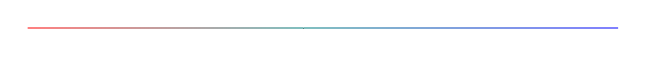
\begin{tikzpicture}
	\fill [left color=red!50, right color=teal!50] (0,0) rectangle (3.5,.01);
	\fill [left color=teal!50, right color=blue!50] (3.5,0) rectangle (7.5,.01);
	\end{tikzpicture}
\vspace{0.5cm}

\begin{example}

.	\vspace{2mm} \textbf{Ejemplo de transformada de Legendre	}

\vspace{2mm} $\boxed{ \ \boldsymbol{f(x) \ = x^2} \ }$

\vspace{2mm} Nueva variable: $\quad p=\displaystyle \dv{f}{x} = f'(x)=2x \ \to \ \boxed{\ x=\dfrac p 2 \ }$

\vspace{2mm} $\displaystyle g(p)=\hat A f(x)=\left[x\dv{x}-1\right] f(x) = \left[x\dv{x}-1\right] \ (x^2) = x(2x)-x^2=2x^2-x^2=x^2=\left( \dfrac p 2 \right)^2= \dfrac{p^2}{4}$

\vspace{2mm} $\boxed{ \boldsymbol{ \ g(p)\ = \dfrac{p^2}{4} } \ }$

\vspace{2mm} Volvamos a plicar $\hat A$ a $g$ para ver si recuperamos la $f$ original.

\vspace{2mm} Nueva variable: $\quad t=\displaystyle \dv{p} g(p) = \dv{p} \left( \dfrac{p^2}{4} \right) =\dfrac p 2 \ \to \ \boxed{\ \boldsymbol{p=2t} \ }$

\vspace{2mm} $h(t)=\hat A g(p) = \displaystyle \left[p\dv{p}-1\right] \ g(p)=\left[p\dv{p}-1\right] \ \dfrac{p^2}{4} = p \dfrac{2p}{4}-\dfrac{p^2}{4}=\dfrac{p^2}{4}=\dfrac{(2t)^2}{4}=t^2$

\vspace{2mm} Por lo que $\quad \boxed{\ \boldsymbol{ h(t)=t^2 \ \leftrightarrow \ h \equiv f } \ }$

$$f(x) \qquad \underrightarrow{\quad \hat{A} \quad} \qquad g(p) \qquad  
\underrightarrow{\quad \hat{A} \quad} \qquad h(t) \equiv f(x)$$

\vspace{2mm} 
\end{example}

\begin{theorem}

 $$f\qquad \underrightarrow{\quad \hat{A} \quad} \qquad g \qquad  
\underrightarrow{\quad \hat{A} \quad}  \qquad f	$$

\vspace{0.1mm}
\end{theorem}
\textcolor{brown}{\rule{200pt}{0.3pt}}

\begin{proof}.
	
\vspace{2mm}	$f(x) \, ; \ \ p=\displaystyle \dv{f}{x} \ \to 	\quad \boldsymbol{g(p)}=\hat A f(x)= \left[x\dv{x}-1\right] f(x)=x\dv{f}{x}-x=\boldsymbol{xp-f}$

\vspace{2mm} $\displaystyle h(q)=\hat A g(p)= \left[p\dv{p}-1\right] g(p) = p\dv{g}{p}-g $

\vspace{2mm} $ \displaystyle \boxed{ \ \displaystyle{h} \ }= \left[p\dv{p}-1\right] g(p)=p\dv{p} \boldsymbol{(xp-f)}- \boldsymbol{(xp-f)}=p\left( \dv{x}{p} p + \bcancel{x \cancelto{1}{\dv{p}{p}}} - \dv{f}{p} \right) - \bcancel{xp} + f=$

$\displaystyle = p \left( \dv{x}{p} p  -\dv{f}{p} \right) + f=\textcolor{gris}{(p=\dv{f}{x})}  =p \left( \dv{x}{p} \cdot \dv{f}{x} - \dv{f}{p} \right) + f = p \left(\dv{f}{p}-\dv{f}{p} \right)+f=p (0) + f =\boxed{ \ \displaystyle{f} \ }$

\end{proof}

\subsection{Una interpretación de la transformada de \emph{Legendre}}
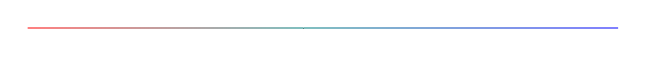
\begin{tikzpicture}
	\fill [left color=red!50, right color=teal!50] (0,0) rectangle (3.5,.01);
	\fill [left color=teal!50, right color=blue!50] (3.5,0) rectangle (7.5,.01);
	\end{tikzpicture}
\vspace{0.5cm}

El razonamiento de Legendre podría haber sido el siguiente:

\begin{multicols}{2}
\begin{figure}[H]
	\centering
	\includegraphics[width=.4\textwidth]{imagenes/img11-01.png}
\end{figure}
$\quad$

Dada una función $f(x)$ y un punto de su dominio $x_0$, llamamos $g$ al punto de corte de la recta tangente a $f(x)$ en $x_0$, $\ y=f'(x_0)(x-x_0)+f(x_0)\, ,$ con el eje de ordenadas ($y$):

$g=-x_of'(x_0)`f(x_0)$. $\quad$ Llamo $p=f'(x_0)\, , $ así:

$g \ = \ -x_0 \, p \ + \ f(x_0) \quad p$ es la pendiente de esta recta.
\end{multicols}

\begin{multicols}{2}
Para otro punto $g$ existirá otra recta tangente a $f$. Teniendo en cuenta todas las posibles pendientes de las rectas tangentes a f(x) tenemos la \emph{transformada de Legendre}. Se trata de encontrar en qué posición del eje $y$ me debo encontrar para lanzar un proyectil desde allí y que sea tangente a $f(x)$. Conocidas todas estad $g$, conoceríamos la \emph{``envolvente''} de la función original y conservaríamos la información que ella guarda.

\begin{figure}[H]
	\centering
	\includegraphics[width=.4\textwidth]{imagenes/img11-02.png}
\end{figure}
\end{multicols}


\begin{multicols}{2}
\begin{figure}[H]
	\centering
	\includegraphics[width=.4\textwidth]{imagenes/img11-03.png}
\end{figure}	
Hemos visto que $\ g=-x_0p+f_0 = \left[ \displaystyle -x\dv{x} +1 \right]\ f$

En termodinámica se define de modo opuesto (un cambio de signo) debido a cuestiones históricas.

Lo podemos reinterpretar como que hay que disparar desde $y>0$ hacia el ej $X$ para que, al rebotar el proyectil en el eje, salga tangente (\emph{rasante}) hacia la función $f(x)$.

\begin{small}\textcolor{gris}{(Transformada de Legendre o los ``disparos rasantes'').}\end{small}

\end{multicols}

\section{Como prodría haber razonado \emph{Hamilton}}
Hamilton conoce el trabajo de Lagrange. Recibe el trabajo de Legendre sobre su transformada y se pregunta qué ocurriría si aplica la transformada al lagrangiano $L$. Obtendré una nueva función que llamaré \emph{hamiltoniano}, $H$, que contendrá la información del lagrangiano: $\subrayado{ \quad \boxed{\ L \qquad \underrightarrow{\quad \hat{A} \quad} \qquad H \ } }$ 


Mecánica clásica 1D (1 dimensión): $\quad L=\dfrac m 2 \dot x^2 - V(x)$

$L(x,\dot x)$, la transformada de Legrendre depende de una sola variable. La variable que nos interesa es $v=\dot x$ que es a la que vamos a aplicar la transformada. Como hay más de una variable, en vez de usar \emph{derivadas totales} usaremos \emph{derivadas parciales}.

$H(p)=\dot A \ L(v)= \left[ v \displaystyle \pdv{v} -1 \right] \ L =\left[ v \displaystyle \pdv{v} -1 \right] \left( \dfrac m 2 v^2 - V(x) \right)$

La nueva variable es $\quad p=\displaystyle \pdv{v} L =mv \ \to \ v=\dfrac p m$

$H(p)=\displaystyle v\pdv{v} (mv^2-V(x)) - (mv^2-V(x))=
v(mv-0)-\dfrac m2 v^2 + V(x)= \dfrac m 2 v^2 + V(x)$

Con la nueva variable,

$H(p)=\displaystyle \dfrac m 2 \left( \dfrac p m \right)^2 + V(x)$

\begin{equation}
H(p) \ = \ \dfrac{p^2}{2m} \ + \ V(x)	
\end{equation}

?`Es $\ H(x,p)\ $ constante en el tiempo?

$\displaystyle \dv{H}{t}=  \dv{H}{p} \dv{p}{t} + \dv{V}{x} \dv{x}{t}=
\dfrac{2p}{2m} \dot p + \dv{V}{x} \dv{x}{t}=\dfrac{p}{m} \dot p + \dv{V}{x} \dot x \qquad $
Como $\quad \dot x=v=\dfrac p m$,

$\displaystyle \dv{H}{t}   
= \dfrac{p}{m} \dot p + \dv{V}{x} \dfrac p m
= \dfrac p m \left[ \dot p + \dv{V}{x} \right]=\dfrac p m \left[ \dot p + V'(x) \right]$

Newton: $\quad	\displaystyle \dot p = - \dv{V}{x} = - V' (x) \ \to \ \dot p +  V' (x)=0$

Por lo que $\quad \displaystyle \dv{H}{t} \ = \ 0 \quad \to \quad H(x,p)=cte \ del \ movimiento$, con dimensiones de \emph{energía}.

Con el Hamiltoniano tenemos otra formulación alternativa a la lagrangiana y, además, aún más potente que ella.



